\documentclass[a4paper,12pt]{article}
\usepackage{amsmath,amsfonts,amssymb}
\usepackage{graphicx}
\usepackage{listings}
\usepackage{xcolor}

\lstset{
    basicstyle=\ttfamily\footnotesize,
    keywordstyle=\color{blue}\bfseries,
    commentstyle=\color{green!60!black},
    stringstyle=\color{red!70!black},
    numbers=none,  % Remove line numbers
    frame=single,
    breaklines=true,
    showstringspaces=false,
    tabsize=4,
    captionpos=b
}

\title{Simulation of Coupled Oscillators}
\author{Abolfazl Mokhtari}

\begin{document}
\maketitle

\section*{General System of $n$ Coupled Oscillators}
The general system consists of \( n \) linearly coupled oscillators without damping. This model is widely applicable to various physical systems such as coupled pendulums, LC circuits, and more. The governing equations are derived using Newton's second law and are numerically solved using the Runge-Kutta method. An animation is generated to visualize the motion of the oscillators.
\\\\The Python code for the general \( n \)-oscillator system is as follows:

\subsection*{Code: General System}
\begin{lstlisting}[language=Python, caption=General system of $n$ coupled oscillators]
import numpy as np
import matplotlib.pyplot as plt
from matplotlib.animation import FuncAnimation

class Oscillator:
    def __init__(self, mass, k_row):
        self.mass = mass
        self.k_row = k_row

def equationOfBlock(oscillator, displacements):
    return (-np.dot(oscillator.k_row, displacements)) / oscillator.mass

def derivatives(t, y, oscillators):
    n = len(oscillators)
    dydt = np.zeros_like(y)
    displacements = y[:n]
    velocities = y[n:]
    dydt[:n] = velocities
    for i in range(n):
        dydt[n + i] = equationOfBlock(oscillators[i], displacements)
    return dydt

def runge_kutta_4(f, y0, t, oscillators):
    n = len(t)
    y = np.zeros((n, len(y0)))
    y[0] = y0
    for i in range(n - 1):
        h = t[i + 1] - t[i]
        k1 = h * f(t[i], y[i], oscillators)
        k2 = h * f(t[i] + h / 2, y[i] + k1 / 2, oscillators)
        k3 = h * f(t[i] + h / 2, y[i] + k2 / 2, oscillators)
        k4 = h * f(t[i] + h, y[i] + k3, oscillators)
        y[i + 1] = y[i] + (k1 + 2 * k2 + 2 * k3 + k4) / 6
    return y

def make_positive_definite(k_matrix):
    eigvals, eigvecs = np.linalg.eigh(k_matrix)
    eigvals[eigvals < 0] = 1e-6
    return eigvecs @ np.diag(eigvals) @ eigvecs.T

def plot_animation(n, masses, k_matrix, initial_displacements, initial_velocities):
    k_matrix = (k_matrix + k_matrix.T) / 2
    k_matrix = make_positive_definite(k_matrix)
    oscillators = [Oscillator(masses[i], k_matrix[i]) for i in range(n)]
    t = np.linspace(0, 20, 1000)
    y0 = np.concatenate([initial_displacements, initial_velocities])
    solution = runge_kutta_4(derivatives, y0, t, oscillators)
    max_amplitude = np.max(np.abs(solution[:, :n]))
    if max_amplitude == 0:
        raise ValueError("All displacement values are zero. Please check the input data.")
    a = max(0.5, 2 * max_amplitude)
    fig, ax = plt.subplots()
    ax.set_xlim(-2, 2 + a * (n - 1))
    ax.set_ylim(-1.5 * max_amplitude, 1.5 * max_amplitude)
    ax.set_aspect('equal', 'box')
    blocks = [plt.Circle((i * a, 0), 0.1, fc='blue') for i in range(n)]
    for block in blocks:
        ax.add_patch(block)
    springs = [ax.plot([], [], 'k-', lw=2)[0] for _ in range(n-1)]
    def init():
        for block in blocks:
            block.set_center((block.center[0], 0))
        for spring in springs:
            spring.set_data([], [])
        return blocks + springs
    def update(frame):
        for i, block in enumerate(blocks):
            block.set_center((a * i + solution[frame, i], 0))
        for i in range(n - 1):
            x = np.linspace(blocks[i].center[0], blocks[i + 1].center[0], 300)
            y = 0.1 * np.sin(60 * (x - blocks[i].center[0]) / (blocks[i + 1].center[0] - blocks[i].center[0]))
            springs[i].set_data(x, y)
        return blocks + springs
    ani = FuncAnimation(fig, update, frames=range(len(t)), init_func=init, blit=True, interval=10)
    plt.show()

# Example:
n = 3
masses = [1, 1, 1]
k_matrix = np.array([
    [2, 1, 0],
    [1, 3, 1],
    [0, 1, 2]
])
initial_displacements = [-1, 0, 1]
initial_velocities = [0, 1, 0]

try:
    plot_animation(n, masses, k_matrix, initial_displacements, initial_velocities)
except ValueError as e:
    print("Error:", e)
\end{lstlisting}

\begin{figure}[h!]
    \centering
    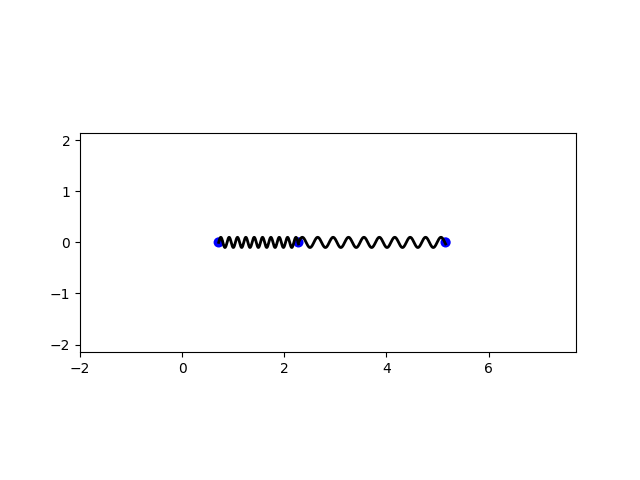
\includegraphics[width=0.8\textwidth]{figures/Figure_1.png}
    \caption{Output of the General System of $n$ Coupled Oscillators}
\end{figure}

\section*{Example: Two Coupled Pendulums with a Spring}
As a specific case, we simulate two pendulums coupled by a spring. The system parameters include the pendulum lengths, gravitational acceleration, and the spring constant. The stiffness matrix for this system is given as:
\[
K = \begin{bmatrix}
\frac{k}{m} + \frac{g}{l} & -\frac{k}{m} \\
-\frac{k}{m} & \frac{k}{m} + \frac{g}{l}
\end{bmatrix}
\]
The initial displacements and velocities are chosen to observe the oscillatory motion.

\subsection*{Code: Two Pendulums}
\begin{lstlisting}[language=Python, caption=Two coupled pendulums]
# Problem data for the two coupled pendulums with a spring
n = 2
m = 1
l = 1
g = 9.8
k = 50

# Stiffness matrix for the two-pendulum system
k_matrix = np.array([
    [k / m + g / l, -k / m],
    [-k / m, k / m + g / l]
])

# Initial conditions
initial_displacements = [0.1, -0.1]
initial_velocities = [0.0, 0.0]

try:
    plot_animation(n, [m] * n, k_matrix, initial_displacements, initial_velocities)
except ValueError as e:
    print("Error:", e)
\end{lstlisting}

\begin{figure}[h!]
    \centering
    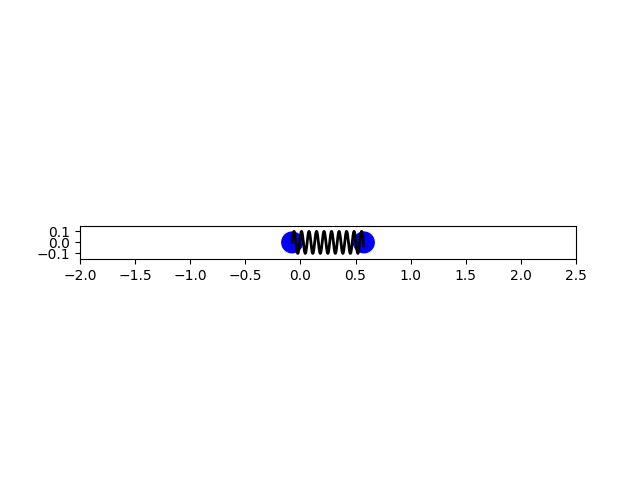
\includegraphics[width=0.8\textwidth]{figures/Figure_2.png}
    \caption{Output of the Two Coupled Pendulums with a Spring}
\end{figure}

\end{document}
